\documentclass[14pt]{extarticle}
\usepackage[T2A]{fontenc}
\usepackage[utf8]{inputenc}
\usepackage[english,bulgarian]{babel}
\usepackage{amssymb,amsmath,stackengine}
\usepackage[margin=0.7in]{geometry}
\usepackage{listings}
\usepackage{float}
\usepackage{caption}
\usepackage[dvipsnames]{xcolor}
\usepackage{hyperref}
\hypersetup{
    colorlinks,
    citecolor=black,
    filecolor=black,
    linkcolor=black,
    urlcolor=black
}
\usepackage{graphicx}
\graphicspath{ {images/} }
\let\frac\dfrac 
\let\epsilon\varepsilon
\renewcommand*\contentsname{СЪДЪРЖАНИЕ}
\newcommand{\me}{\mathrm{e}}
\newcommand{\mi}{\mathrm{i}}
\lstset{basicstyle=\footnotesize\ttfamily,breaklines=true}
\lstset{language=Matlab,
    %basicstyle=\color{red},
    breaklines=true,%
    frame=single,
    morekeywords={matlab2tikz},
    keywordstyle=\color{blue},
    morekeywords=[2]{1}, keywordstyle=[2]{\color{black}},
    identifierstyle=\color{black},
    stringstyle=\color{purple},
    commentstyle=\color{ForestGreen},
    showstringspaces=false,%without this there will be a symbol in the places where there is a space
    numbers=left,
    numberstyle={\tiny \color{black}},% size of the numbers
    numbersep=10pt, % this defines how far the numbers are from the text
    %emph=[1]{for,end,break},emphstyle=[1]\color{red}, %some words to emphasise
    %emph=[2]{word1,word2}, emphstyle=[2]{style},    
}
 
\begin{document}
  
\begin{center}


\includegraphics{fmi}

\vspace{1cm}

{\large \textbf{П Р О Е К Т}}\\
по\\
\textbf{Диференциални уравнения и приложения}\\
спец. Софтуерно инженерство, 2 курс, летен семестър,\\
учебна година 2015/16\\
\textbf{Тема №3}\\

\vspace{2cm}
Изготвил: Антон Александров Петков\\
Фак. №: 61793\\
Група: 1\\

\vspace{1cm}
05.06.2016 гр. София

\end{center}


\vfill\hfill
Оценка:..............................

\newpage
 
\tableofcontents

\section{Тема (задание) на проекта}

\begin{center}
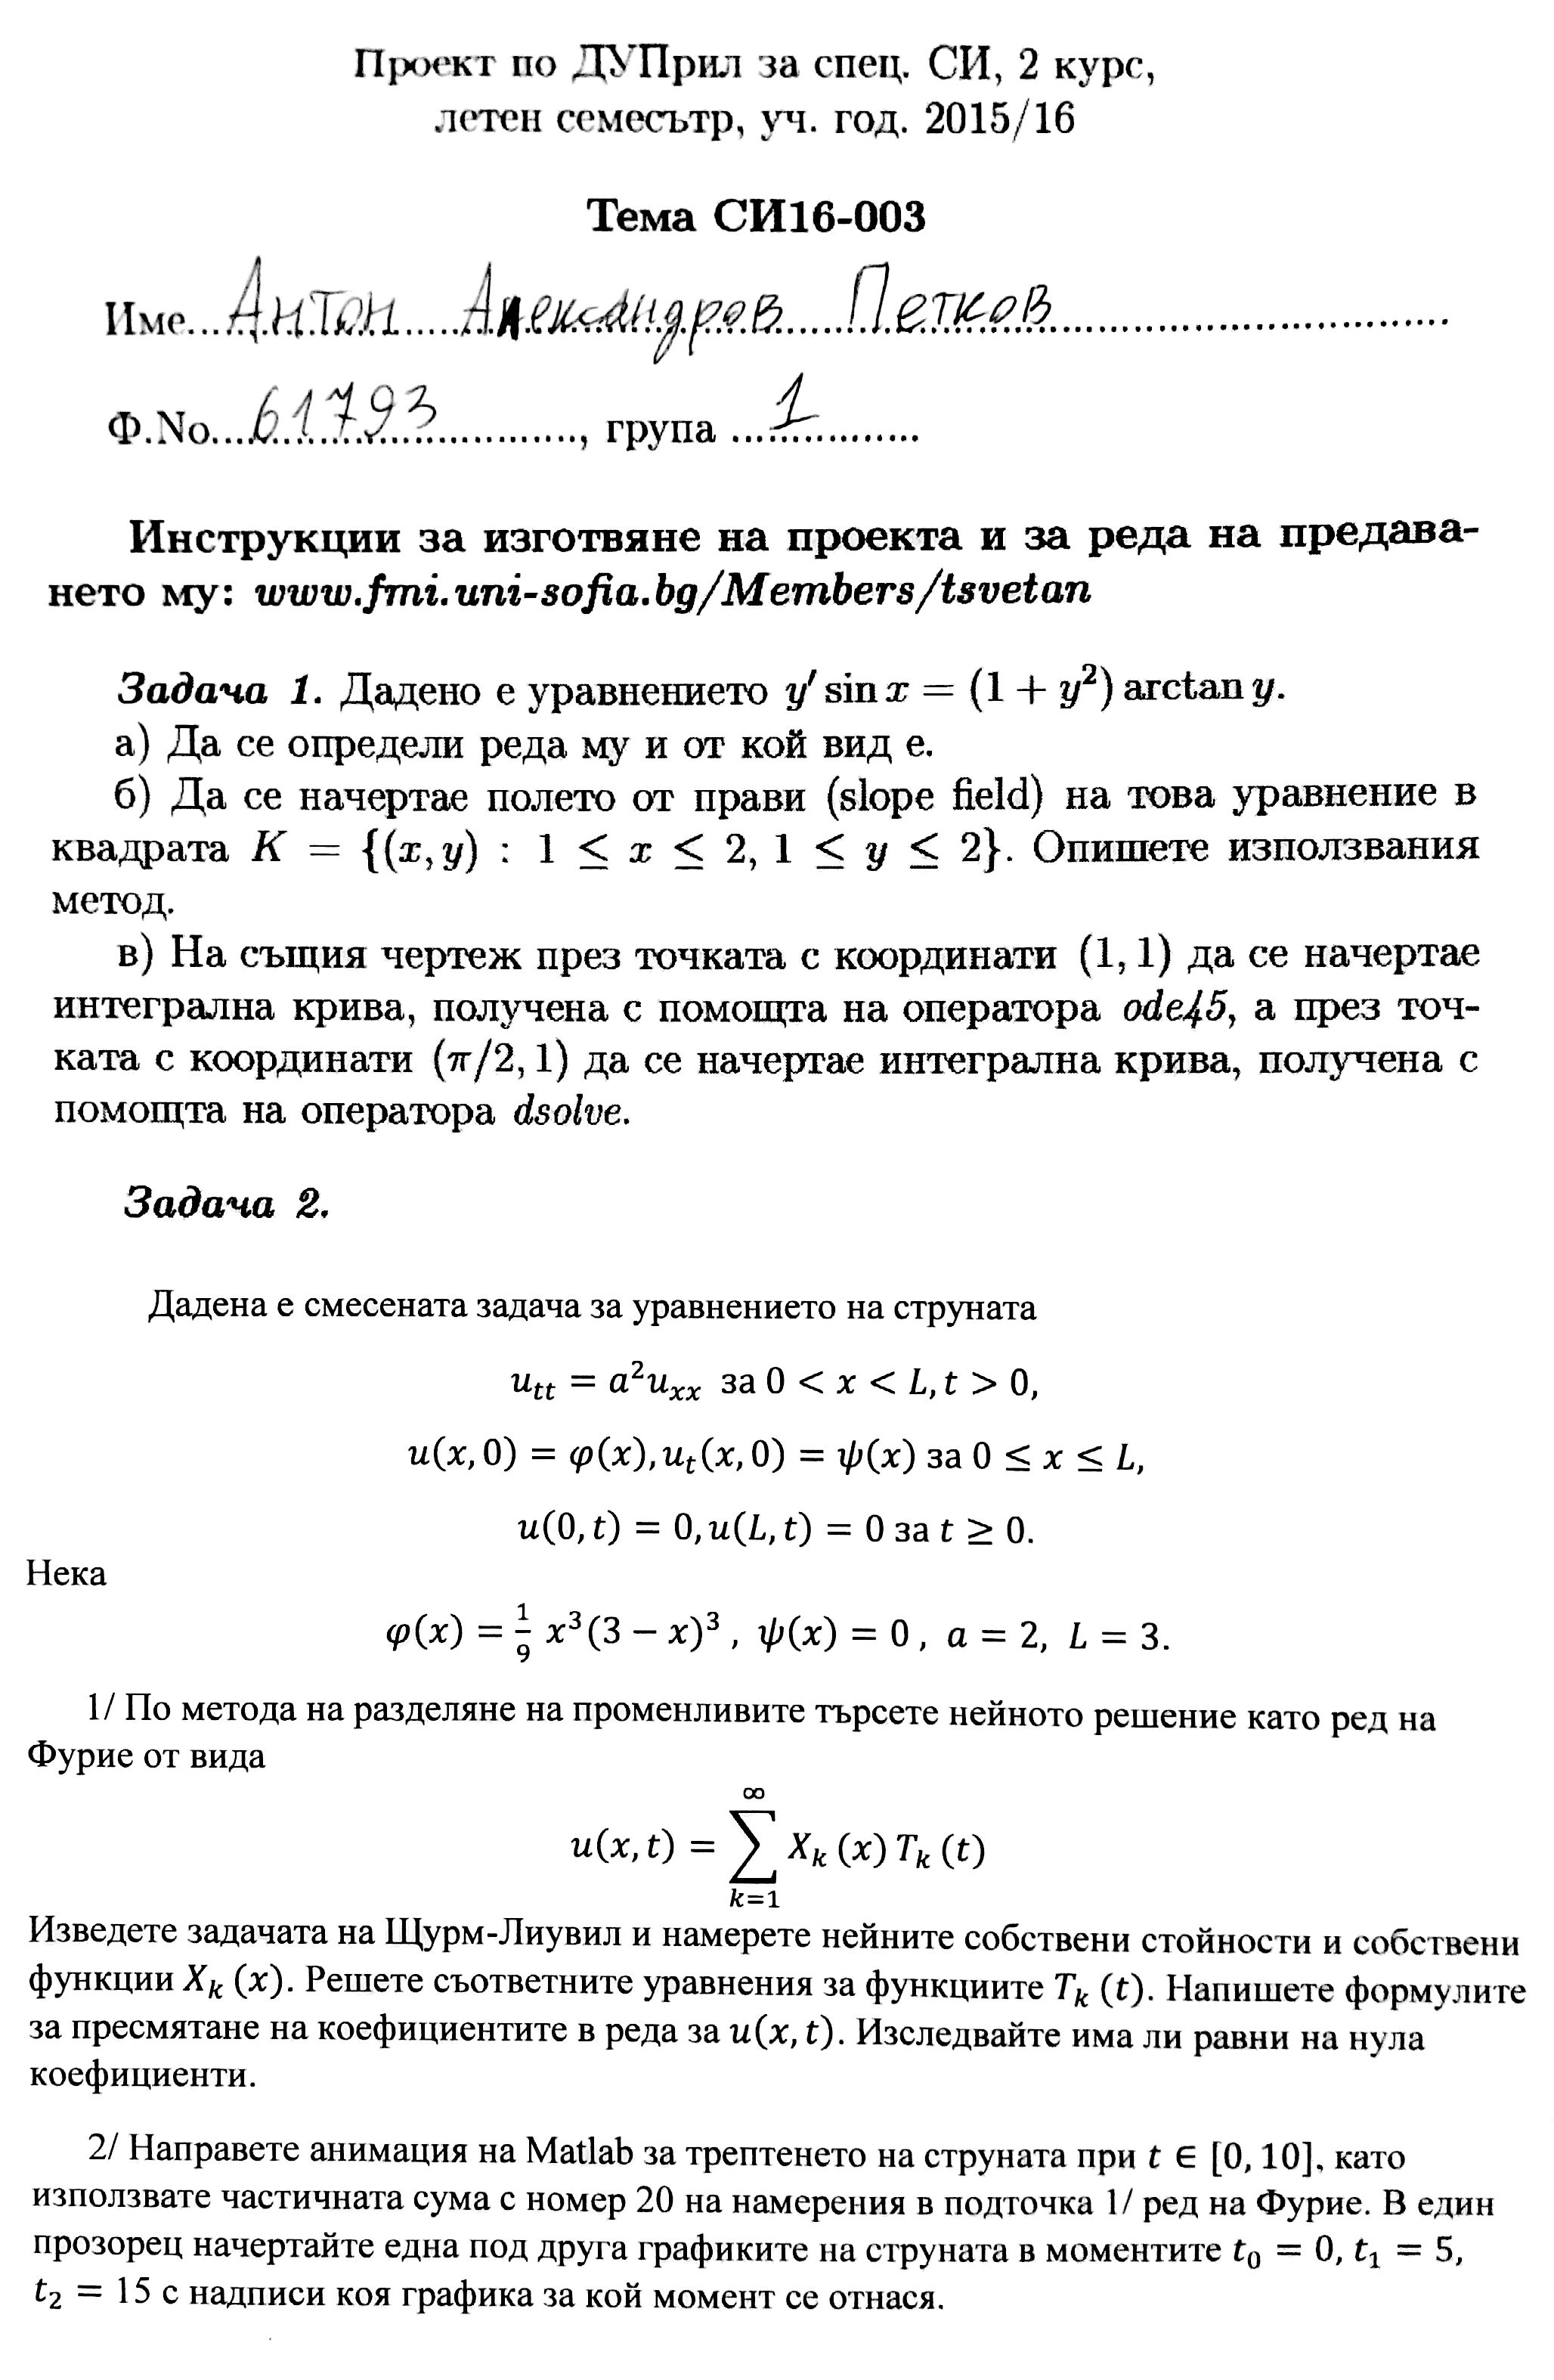
\includegraphics[width=0.9\textwidth,height=0.9\textheight,keepaspectratio]{instructions}
\end{center}

\section{Решение на Задача 1.}

\begin{equation}
	\displaystyle y'\sin x = (1+y^2)\arctan y \tag{1}\label{eq:1}
\end{equation}

\[
y =
\left\{
	\begin{array}{ll}
		\tg c | \tg \tfrac{x}{2} |  & \mbox{при } y \geq 0 \\
		-\tg c | \tg \tfrac{x}{2} | & \mbox{при } y < 0
	\end{array}
\right.
\]

\begin{center}
Където $ c = const $.
\end{center}

\textbf{a)} Диференциалното уравнение \eqref{eq:1} е обикновенно диференциално уравнение от първи ред с разделящи се променливи.

\subsection{Теоретична част}

\[ \int \frac{dy}{(1+y^2)\arctan y} = \int \frac{dx}{\sin x} \]

Решаваме лявата част от уравнението \eqref{eq:1}, вкарвайки $\tfrac{1}{1 + y^2}$ зад диференциала.

\[ \int \frac{dy}{(1+y^2)\arctan y} = \int \frac{d(\arctan y)}{\arctan y} = \ln | \arctan y | + c_1  \]\newline

Дясната част на \eqref{eq:1} решаваме чрез универсална субституция.

\[ u = \tg \tfrac{x}{2}, \hspace{5mm} x = 2\arctan u, \hspace{5mm} dx = \frac{2du}{1+u^2}\]

\[ \sin x = \frac{2 \tg \tfrac{x}{2}}{1 + \tg^2 \tfrac{x}{2}} = \frac{2u}{1+u^2} \]

\[ \int \frac{dx}{\sin x} = \int \frac{1+u^2}{2u} \cdot \frac{2du}{1+u^2} = \int \frac{du}{u} = \ln | \tg \tfrac{x}{2} | + c_2 \]\newline

\[ \ln | \arctan y | + c_1 =  \ln | \tg \tfrac{x}{2} | + c_2  \]

Полагаме $c_3 = c_2 - c_1$ и правим разлика на логаритмите.

\[ \ln \frac{| \arctan y |}{| \tg \tfrac{x}{2} |} =  c_3  \]

Нека $c_4 = \me^{c_3}$.

\[ \frac{| \arctan y |}{| \tg \tfrac{x}{2} |} = c_4 \]

\[ | \arctan y | = c_4 | \tg \tfrac{x}{2} | \]

Прилагаме тангенс от двете страни, спазвайки ограничението на левия модул.

\[
y =
\left\{
	\begin{array}{ll}
		\tg c_4 | \tg \tfrac{x}{2} |  & \mbox{при } y \geq 0 \\
		-\tg c_4 | \tg \tfrac{x}{2} | & \mbox{при } y < 0
	\end{array}
\right.
\]\newline

\textbf{Поле от прави}

Нека $y' = f(x, y)$ и нека имаме мрежа от точки с координати $(x_k, y_k)$. За да начертаем права, минаваща през точката $(x_k, y_k)$ с ъглов коефициент $s$ използваме уравнението $y-y_0 = s(x - x_0)$, където ъгловият коефициент $s = y'(x_k) = f(x_k, y_k) = \tg\varphi$, а $\varphi$ е ъгълът между правата и абсцисната ос.

Избираме някое $\delta > 0$ такова, че дължината на отсечка от полето от прави е $2\delta$. Нека $\epsilon > 0$ е такова, че $2\epsilon$ е дължината на проекцията на отсечката от полето от прави. Така $\tg\varphi = \frac{\sqrt{\delta^2 - \epsilon^2}}{\epsilon}$. За произволна точка $(x_k, y_m)$ от мрежата от точки ще изразим $\epsilon > 0$:

\[ \epsilon f(x_k, y_m) = \sqrt{\delta^2 - \epsilon^2} \]

\[ \epsilon^2f^2(x_k, y_m) = \delta^2 - \epsilon^2 \]

\[ \epsilon^2 = \frac{\delta^2}{1 + f^2(x_k, y_m)} \]

\[ \epsilon = \frac{\delta}{\sqrt{1 + f^2(x_k, y_m)}} \]

Така двете точки $(x_k-\epsilon, y_m - \epsilon f(x_k, y_m)) , \, (x_k+\epsilon, y_m + \epsilon f(x_k, y_m))$ определят краищата на отсечка от полето от прави.

\subsection{MATLAB  код и получени в командния прозорец резултати при изпълнението му}

\begin{figure}[H]
	\begin{quote}
	\lstinputlisting[language=MATLAB]{code/task1.m}
	\end{quote}
	\caption{Код на решението на първа задача.}
\end{figure}

\subsection{Графики (включително от анимация)}

\begin{figure}[H]
	\centering
	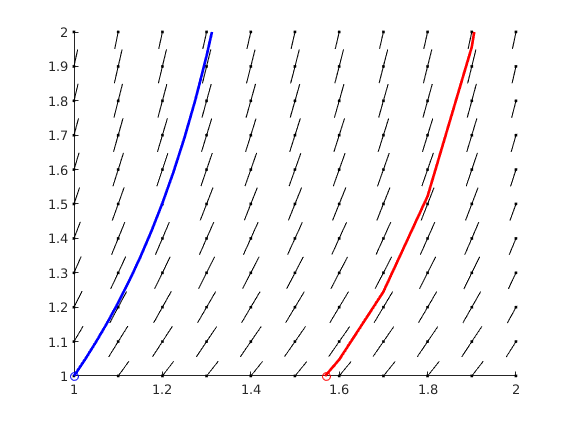
\includegraphics{images/task1}
	\caption{Илюстрация на решението на първа задача.}
\end{figure}

\subsection{Коментари към получените с MATLAB резултати}

На Фигура 2 с черен цвят е изобразено полето от прави за уравнение \eqref{eq:1}.
В точка (1, 1) започва в син цвят интегралната крива, получена с помощта на оператора \textbf{ode45}, а през точката с координати $\left(\frac{\pi}{2},1\right)$ с червен цвят е начертана интегралната крива, получена с помощта на оператора \textbf{dsolve}.

\section{Решение на Задача 2.}

\[
\left\{
	\begin{array}{ll}
		\displaystyle u(x,t) = \sum_{k=1}^{\infty} \left( A_k\cos\frac{ak\pi}{L}t + B_k\sin\frac{ak\pi}{L}t \right) \sin\frac{k\pi}{L}x \\
		\displaystyle A_k = \frac{2}{L} \int_0^L \frac{1}{9}x^3(3-x)^3 \sin\frac{k\pi}{L}x \, dx \\
		B_k = 0
	\end{array}
\right.
\]

\subsection{Теоретична част}

Търсим решение от вида $u(x,t) = X(x)T(t) \not\equiv 0$.

\[ X(x)T''(t) = a^2X''(x)T(t) \]

\[ \frac{T''(t)}{a^2T(t)} = \frac{X''(x)}{X(x)} = -\lambda , \hspace{1cm} \mbox{където } \lambda = const \]

\[ T''(t) + \lambda a^2T(t) = 0 , \hspace{1cm} t \geq 0 \]
\[ X''(x) + \lambda X(x) = 0 , \hspace{1cm} 0 \leq x \leq L \]

От граничните условия:

\[ u \big|_{x=0} = X(0)T(t) = 0 , t \geq 0 \implies X(0) = 0 \]
\[ u \big|_{x=L} = X(L)T(t) = 0 , t \geq 0 \implies X(L) = 0 \]

За $X(x)$ получаваме задачата на Щурм-Лиувил:

\begin{equation}
\left\{
	\begin{array}{ll}
		X''(x) + \lambda X(x) = 0 & , 0 < x < L \\ \tag{2}\label{eq:2}
		X(0) = 0, X(L) = 0
	\end{array}
\right.
\end{equation}

Търсим ненулево решение на уравнението \eqref{eq:2}, което е линейно. Характерситияният полином на \eqref{eq:2} е $P(\alpha) = \alpha^2 + \lambda = 0 \implies \alpha^2 = -\lambda$.

\noindent 1) ако $\lambda < 0$

$ \alpha_1 = -\sqrt{-\lambda}, \hspace{2mm} \alpha_2 = \sqrt{-\lambda} $

Фундаменталната система решения е $\{\me^{-\sqrt{-\lambda}x}, \me^{\sqrt{-\lambda}x}\}$.

$X(x) = c_1\me^{-\sqrt{-\lambda}x} + c_2\me^{\sqrt{-\lambda}x}$

$X(0) = c_1 + c_2 = 0 \implies c_2 = -c_1$

$X(L) = c_1\left( \me^{-\sqrt{-\lambda}L} - \me^{\sqrt{-\lambda}L} \right) \implies c_1 = 0 \implies X(x) = 0$

\noindent 2) ако $\lambda = 0$

$ \alpha_1 = \alpha_2 = 0 $

Фундаменталната система решения е $\{1, x\}$.

$X(x) = c_1x + c_2$

$X(0) = c_2 = 0$

$X(L) = c_1L = 0 \implies c_1 = 0 \implies X(x) = 0$

\noindent 3) ако $\lambda > 0$

$ \alpha_1 = -\mi\sqrt{\lambda}, \hspace{2mm} \alpha_2 = \mi\sqrt{\lambda} $

Фундаменталната система решения е $\{ \cos \sqrt{\lambda}x, \sin \sqrt{\lambda}x \}$.

$X(x) = c_1\cos \sqrt{\lambda}x + c_2\sin \sqrt{\lambda}x$

$X(0) = c_1 \cos 0 = c_1 = 0$

\begin{equation}
X(L) = c_2\sin\sqrt{\lambda}L = 0 \tag{3}\label{eq:3}
\end{equation}

Равенство \eqref{eq:3} е възможно при $c_2 = 0$ или при $\sin\sqrt{\lambda}L = 0$, което се случва само при $\sqrt{\lambda}L = k\pi$ за $k \in \mathbb{N}$.

Собствените стойности на задачата на Щурм-Лиувил са $\lambda_k = \left( \frac{k\pi}{L} \right)^2 , k \in \mathbb{N}$.

А собствените функции са $X_k(x) = \sin \left( \frac{k\pi x}{L} \right) , k \in \mathbb{N}$.

Нека $\lambda = \lambda_k$. Ще решим уравненията за $T_k(t)$.

$ T_k''(t) + \left( \frac{ak\pi}{L} \right)^2T_k(t) = 0 $

Характеристичният полином е $ P_k(\alpha) = \alpha^2 + \left( \frac{ak\pi}{L} \right)^2 = 0$.

Корените са $\alpha_1 = -\frac{ak\pi}{L}, \hspace{2mm} \alpha_2 = \frac{ak\pi}{L}$.

Фундаменталната система решения е $\{ \cos\frac{ak\pi}{L}, \sin\frac{ak\pi}{L} \}$.

$T_k(t) = A_k\cos\frac{ak\pi}{L} + B_k\sin\frac{ak\pi}{L}$

Получихме функции $u_k(x,t) = T_k(t)X_k(t)$, които са решението на уравнението на струната и удовлетворяват граничните условия.

Избираме коефициентите $A_k$ и $B_k$:

$\displaystyle A_k = \frac{2}{L} \int_0^L \varphi(x)\sin\frac{k\pi x}{L} dx$

$\displaystyle B_k = \frac{2}{ak\pi} \int_0^L \psi(x)\sin\frac{k\pi x}{L} dx$, но понеже $\psi(x) = 0 \implies B_k = 0$.

\subsection{MATLAB  код и получени в командния прозорец резултати при изпълнението му}

\begin{figure}[H]
	\begin{quote}
	\lstinputlisting[language=MATLAB]{code/task21.m}
	\end{quote}
	\centering
	\caption{Код за анимацията на трептенето на струната от втора задача.}
\end{figure}

\begin{figure}[H]
	\centering
	\captionsetup{justification=centering,margin=2cm}
	\begin{quote}
	\lstinputlisting[language=MATLAB]{code/task22.m}
	\end{quote}
	\caption{Код за начертаването на графиките на струната\\в моментите $t_0 = 0, t_1 = 5, t_2 = 15$.}
\end{figure}

\subsection{Графики ( включително от анимация)}

\begin{figure}[H]
	\captionsetup{justification=centering,margin=2cm}
	\centering
	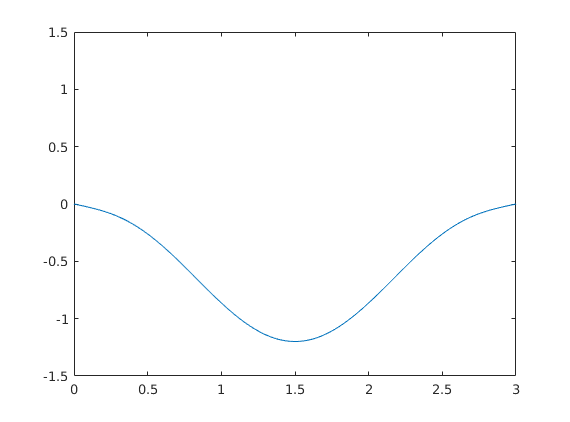
\includegraphics[scale=0.8]{images/task21down}
	\caption{Анимация на трептенето на струната в момента, когато струната е най-ниско.}
\end{figure}

\begin{figure}[H]
	\captionsetup{justification=centering,margin=2cm}
	\centering
	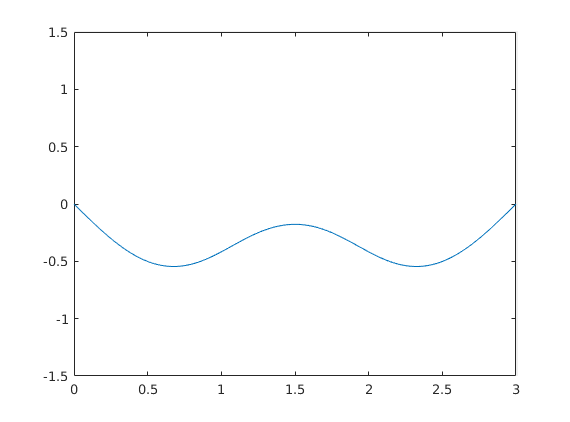
\includegraphics[scale=0.8]{images/task21downMid}
	\caption{Анимация на трептенето на струната в момента, когато струната се измества от най-ниското си положение към центъра.}
\end{figure}

\begin{figure}[H]
	\captionsetup{justification=centering,margin=2cm}
	\centering
	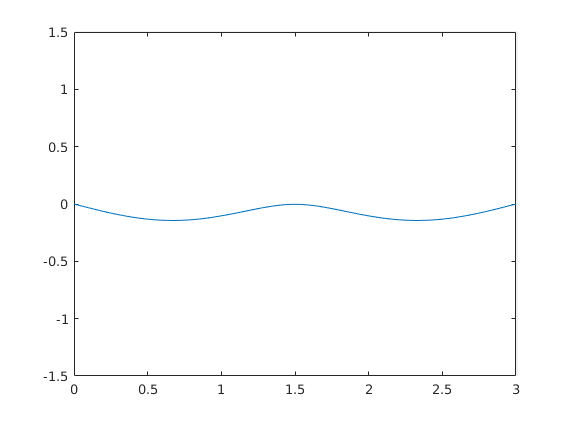
\includegraphics[scale=0.8]{images/task21mid}
	\caption{Анимация на трептенето на струната в момент, когато е близко до равновесното си положение.}
\end{figure}

\begin{figure}[H]
	\captionsetup{justification=centering,margin=2cm}
	\centering
	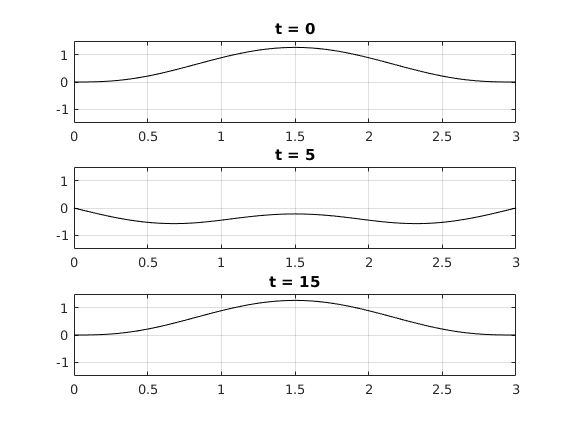
\includegraphics{images/task22moments}
	\caption{Илюстрация на трептенето на струната\\в трите момента $t_0 = 0, t_1 = 5, t_2 = 15$.}
\end{figure}


\subsection{Коментари към получените с MATLAB резултати}
\hspace{7mm}На фигури 5, 6 и 7 се виждат кадри от анимацията на трептенето на струната.
Първоначално струната застава в най-високото си положение, максимално далеч от равновесното си положение, като има един глобален максимум. Постепенно се прибира надолу към равновесното си положение, като има момент в който функцията има 3 локални екстремума, два от които са локални максимуми. След като струната премине равновесното си положение, тя минава последователно през състоянията илюстрирани съответно на фигури 7, 6 и 5, като на фигура 5 достига най-ниската си точка, отново максимално отдалечена от равновесното си състояние.

На Фигура 8 е изобразено трептенето на струната в моментите $t_0 = 0, t_1 = 5, t_2 = 15$. Струната е идентична в моментите $t_0$ и $t_2$ - има един глобален максимум. Докато в момент $t_1$ струната е по-вълнообразна и има три локални екстремума.

\end{document}